\usepackage{fontspec}

\setsansfont{Montserrat}
\newfontfamily\caps{Montserrat}[Kerning=Uppercase]
\let\familydefault\sfdefault

\usepackage{xcolor}
\usepackage{tikz}
\usetikzlibrary{decorations.text}
\pgfdeclarelayer{back}
\pgfsetlayers{back,main}

\usepackage{xifthen}
\usepackage{calc}

\raggedright
\usepackage{xparse}

\definecolor{darkBlue}{RGB}{15, 74, 144}
\definecolor{lightBlue}{RGB}{69, 144, 197}


\nopagecolor
\pagestyle{empty}

\NewDocumentCommand \laenderlogo {O{30} m} {%
  \fontsize{30}{30}\selectfont%
  \begin{tikzpicture}%
    \fill[fill=white] (0, 0) circle (3.4cm);
    \fill[fill=lightBlue, even odd rule]
      (0, 0) circle (5cm)
      (0, 0) circle (3.4cm);

    \begin{scope}
      \clip (0, 0) circle (3.34cm);
      \node[anchor=center] at (0, 0) {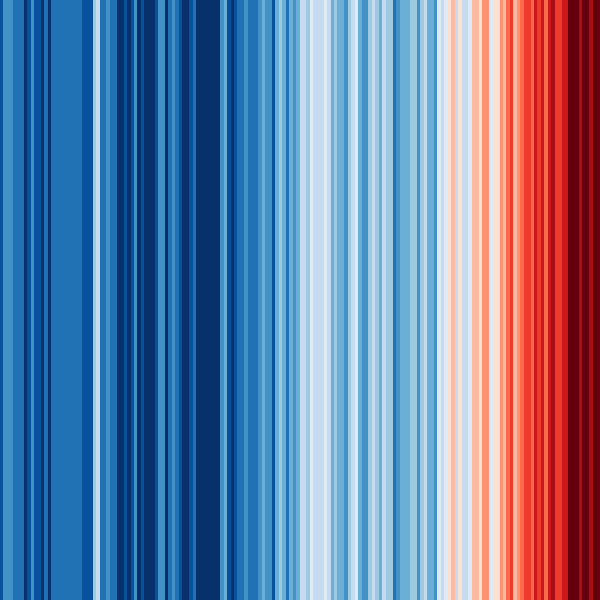
\includegraphics[height=6.68cm]{warming_stripes.pdf}};
    \end{scope}

    \path[
      postaction={
        decorate,
        decoration={
          text along path,
          text align=center,
          text color=white,
          raise=-0.4em,
          text={|\bfseries\caps|SCIENTISTS FOR FUTURE},
        }
      },
    ] (225:4.2cm) arc [start angle=225, end angle=45, radius=4.2cm];

    \fontsize{#1}{#1}\selectfont
    \path[
      postaction={
        decorate,
        decoration={
          text along path,
          text align=center,
          text color=white,
          raise=-0.4em,
          text={|\bfseries\caps|#2},
        }
      },
    ] (240:4.2cm) arc [start angle=240, end angle=390, radius=4.2cm];
  \end{tikzpicture}%
}

\newlength\namewidth

\NewDocumentCommand \laenderbanner {s O{30} m m} {{%
  \fontsize{18}{18}\selectfont\bfseries%
  \newcommand\groupname{%
    \fontsize{24}{24}\selectfont\bfseries #3%
  }%
  \setlength{\namewidth}{\widthof{\groupname}}%
  \newcommand\sff{%
    Scientists \textcolor{lightBlue}{for} Future%
  }

  \begin{tikzpicture}[
      inner sep=0.2cm, outer sep=0,
    ]%

    % alignment of group name depending on its size
    % either aligned with Future or if too broad, right aligned
    \coordinate (name) at (6.87, 0.1);
    \tikzset{groupname/.style={anchor=south west, text=lightBlue, inner sep=0.2cm, outer sep=0}};
    \useasboundingbox (0,0) rectangle (6.87cm + \namewidth + 0.4cm, 2.5cm);
    \clip (0,0) rectangle (6.87cm + \namewidth + 0.4cm, 2.5cm);


    \tikzset{padding/.style={fill=white, rounded corners}}

    \node[inner sep=0] (logo) at (1.2, 1.3) {%
      \resizebox{2cm}{2cm}{\laenderlogo[#2]{#4}}%
    };
    \node[anchor=west, xshift=0.3em, yshift=0.5ex, text=darkBlue] (s4) at (logo.east) {\sff};
    \node[groupname] at (name) {\groupname};

    % draw white padding if * is given
    \IfBooleanT{#1}{
      \begin{pgfonlayer}{back}
        \fill[white] (logo.center) circle (1.2);
        \node[groupname, padding] at (name) {\phantom{\groupname}};

        \node[padding, anchor=west, xshift=0.3em, yshift=0.5ex] (s4) at (logo.east) {\phantom{\sff}};
      \end{pgfonlayer}
    }
  \end{tikzpicture}%
}}
